%%%%%%%%%%%%%%%%%%%%%%%%%%%%%%%%%%%%%%%%%
% Short Sectioned Assignment LaTeX Template Version 1.0 (5/5/12)
% This template has been downloaded from: http://www.LaTeXTemplates.com
% Original author:  Frits Wenneker (http://www.howtotex.com)
% License: CC BY-NC-SA 3.0 (http://creativecommons.org/licenses/by-nc-sa/3.0/)
%%%%%%%%%%%%%%%%%%%%%%%%%%%%%%%%%%%%%%%%%

%----------------------------------------------------------------------------------------
%	PACKAGES AND OTHER DOCUMENT CONFIGURATIONS
%----------------------------------------------------------------------------------------

\documentclass[paper=a4, fontsize=11pt]{scrartcl} % A4 paper and 11pt font size

% ---- Entrada y salida de texto -----

\usepackage[T1]{fontenc} % Use 8-bit encoding that has 256 glyphs
\usepackage[utf8]{inputenc}
%\usepackage{fourier} % Use the Adobe Utopia font for the document - comment this line to return to the LaTeX default

% ---- Idioma --------

\usepackage[spanish, es-tabla]{babel} % Selecciona el español para palabras introducidas automáticamente, p.ej. "septiembre" en la fecha y especifica que se use la palabra Tabla en vez de Cuadro

% ---- Otros paquetes ----

\usepackage{url} % ,href} %para incluir URLs e hipervínculos dentro del texto (aunque hay que instalar href)
\usepackage{hyperref}
\hypersetup{
	colorlinks=true,
	linkcolor=black,
	urlcolor=black,
	citecolor=black,
}
\usepackage{amsmath,amsfonts,amsthm} % Math packages
%\usepackage{graphics,graphicx, floatrow} %para incluir imágenes y notas en las imágenes
\usepackage{graphics,graphicx, float} %para incluir imágenes y colocarlas

% Para hacer tablas comlejas
%\usepackage{multirow}
%\usepackage{threeparttable}

%\usepackage{sectsty} % Allows customizing section commands
%\allsectionsfont{\centering \normalfont\scshape} % Make all sections centered, the default font and small caps

\usepackage{fancyhdr} % Custom headers and footers
\pagestyle{fancyplain} % Makes all pages in the document conform to the custom headers and footers
\fancyhead{} % No page header - if you want one, create it in the same way as the footers below
\fancyfoot[L]{} % Empty left footer
\fancyfoot[C]{} % Empty center footer
\fancyfoot[R]{\thepage} % Page numbering for right footer
\renewcommand{\headrulewidth}{0pt} % Remove header underlines
\renewcommand{\footrulewidth}{0pt} % Remove footer underlines
\setlength{\headheight}{13.6pt} % Customize the height of the header

\numberwithin{equation}{section} % Number equations within sections (i.e. 1.1, 1.2, 2.1, 2.2 instead of 1, 2, 3, 4)
\numberwithin{figure}{section} % Number figures within sections (i.e. 1.1, 1.2, 2.1, 2.2 instead of 1, 2, 3, 4)
\numberwithin{table}{section} % Number tables within sections (i.e. 1.1, 1.2, 2.1, 2.2 instead of 1, 2, 3, 4)

\setlength\parindent{0pt} % Removes all indentation from paragraphs - comment this line for an assignment with lots of text

\newcommand{\horrule}[1]{\rule{\linewidth}{#1}} % Create horizontal rule command with 1 argument of height
\usepackage{booktabs}

\usepackage{listings}
\lstdefinelanguage
[x64]{Assembler}     % add a "x64" dialect of Assembler
[x86masm]{Assembler} % based on the "x86masm" dialect
{morekeywords={CDQE,CQO,CMPSQ,CMPXCHG16B,JRCXZ,LODSQ,MOVSXD, %
		POPFQ,PUSHFQ,SCASQ,STOSQ,IRETQ,RDTSCP,SWAPGS, %
		rax,rdx,rcx,rbx,rsi,rdi,rsp,rbp, %
		r8,r8d,r8w,r8b,r9,r9d,r9w,r9b, %
		r10,r10d,r10w,r10b,r11,r11d,r11w,r11b, %
		r12,r12d,r12w,r12b,r13,r13d,r13w,r13b, %
		r14,r14d,r14w,r14b,r15,r15d,r15w,r15b}} % etc.
\usepackage{color}
\usepackage{xcolor}
\lstdefinestyle{customc}{
	belowcaptionskip=1\baselineskip,
	breaklines=true,
	frame=L,
	xleftmargin=\parindent,
	language=C,
	showstringspaces=false,
	basicstyle=\footnotesize\ttfamily,
	keywordstyle=\bfseries\color{green!40!black},
	commentstyle=\itshape\color{purple!40!black},
	identifierstyle=\color{blue},
	stringstyle=\color{orange},
}

\lstset{escapechar=@,style=customc}
\usepackage{url}

\title{	
	\normalfont \normalsize
	\begin{figure}[htb]
		\centering
		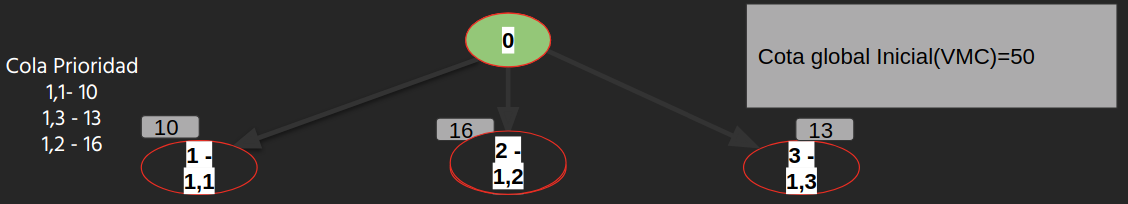
\includegraphics[width=0.3\textwidth]{./imagenes/1}
	\end{figure}
	\textsc{\textbf{Algoritmica} \\ Grado en Ingeniería Informática \\ 
	Curso 2018-2019} \\ [25pt] 
	\begin{figure}[htb]
		\centering
		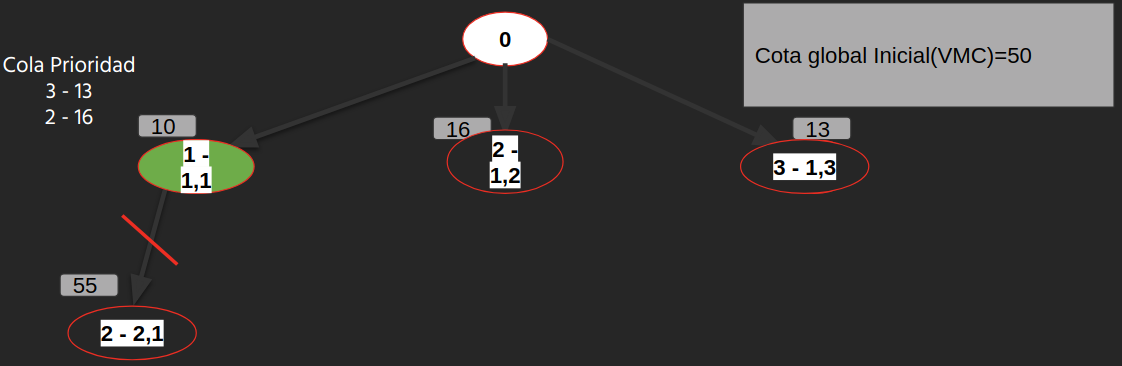
\includegraphics[width=0.15\textwidth]{./imagenes/2}
	\end{figure}
	\horrule{0.5pt} \\[0.4cm]
	\huge Ejercicio Propuesto 1. \\
	\huge Principio de Invarianza.
	\\ 
	\horrule{2pt} \\[0.5cm] 
}
\author{Félix Ramírez García  \\
\href{mailto:felixramirezgarcia@correo.ugr.es}{felixramirezgarcia@correo.ugr.es}}
\date{\normalsize\today} 

%----------------------------------------------------------------------------------------
% DOCUMENTO
%----------------------------------------------------------------------------------------

\begin{document}
	
	\maketitle % Muestra el Título
	
	\newpage %inserta un salto de página
	
	\tableofcontents % para generar el índice de contenidos
	
	\listoffigures % para generar índice de imágenes.
	
	\listoftables % para generar índice de tablas.
	
	\newpage
	
	%-----------------------------------------------------------------------
	%							Introduccion
	%----------------------------------------------------------------------	
	\section[Introduccion]{Introduccion}
		
	El enunciado del ejercicio nos propone usar los programas BurbujaC.cpp y BurbujaJava.java para ilustrar el cumplimiento del principio de invariaza. Para ello ejecutaremos la misma función en ambos programas con diferentes tamaños del problema anotando sus tiempos de ejecucion para comparar los resultados gráficamente. \\
	
	Recordemos que el principio de invarianza plantea que dos versiones del mismo algoritmo no difieren en su eficiencia en más que una constante. Por lo que al ejecutar los dos programas obtendremos un resultado similar independientemente de la maquina y del lenguaje de programación usado.\\ 
	
	Empezando con el siguiente programa en C++ (BurbujaC.cpp) que ordena una lista desordenada en orden inverso (peor caso) de 20.000 numeros , cada 1000 (se ordenan 20 arrays), compilado y ejecutado con las ordenes : \\
	
	g++ -o BurbujaC.cpp BurbujaC\\
	./BurbujaC
	
	\lstset{language=C}
	\begin{lstlisting}[frame=single] 
#include <iostream>
#include <ctime>
using namespace std;

void Burbuja(double *v, int posini, int posfin) {
	int i, j;
	double aux;
	bool haycambios= true;	
	i= posini;
	
	while (haycambios) {	
		haycambios=false; // Suponemos vector ya ordenado
		
		// Recorremos vector de final a i
		for (j= posfin; j>i; j--) {
		
			// Dos elementos consecutivos mal ordenados
			if (v[j-1]>v[j]) {
				aux= v[j]; // Los intercambiamos
				v[j]= v[j-1];
				v[j-1]= aux;
				
				// Al intercambiar, hay cambio
				haycambios= true;
			}
		}
		
		i++;
	}
}


int main()
{
	const int SIZE= 20000;
	double vect[SIZE];
	unsigned long tini, tfin;
	
	for (int TAM= 1000; TAM<=SIZE; TAM+= 1000) {	
		// Ejemplo: Vector al reves
		for (int i= 0; i<TAM; i++)
		vect[i]= TAM-i;
		
		tini= clock(); // Tiempo inicial
		Burbuja(vect, 0, TAM-1);
		tfin= clock(); // Tiempo final
		
		cout<<"N: "<<TAM<<" T (ms.): "<<1000.0*(tfin-tini)/(double)CLOCKS_PER_SEC<<endl;
	}
	return 0;
}
	\end{lstlisting}
	
	Obtenemos la siguiente salida :\\
	
	\lstset{language=C}
	\begin{lstlisting}[frame=single]
N: 1000 T (ms.): 0
N: 2000 T (ms.): 15.625
N: 3000 T (ms.): 31.25
N: 4000 T (ms.): 62.5
N: 5000 T (ms.): 93.75
N: 6000 T (ms.): 140.625
N: 7000 T (ms.): 234.375
N: 8000 T (ms.): 312.5
N: 9000 T (ms.): 328.125
N: 10000 T (ms.): 421.875
N: 11000 T (ms.): 609.375
N: 12000 T (ms.): 656.25
N: 13000 T (ms.): 671.875
N: 14000 T (ms.): 812.5
N: 15000 T (ms.): 937.5
N: 16000 T (ms.): 1156.25
N: 17000 T (ms.): 1250
N: 18000 T (ms.): 1421.88
N: 19000 T (ms.): 1406.25
N: 20000 T (ms.): 1656.25
	\end{lstlisting} 
	
	Y para una mejor visualización representamos los resultados en una gráfica (figura 1.1).\\
	
	\begin{figure}[htb]
		\centering
		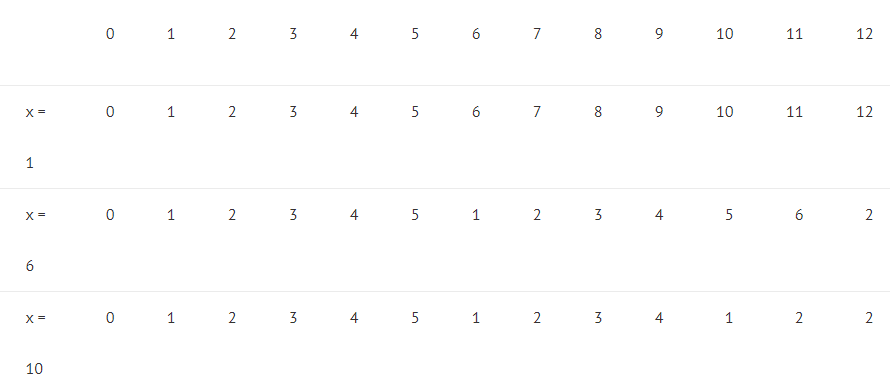
\includegraphics[width=1.0\textwidth]{./imagenes/3}
		\caption{Grafica BurbujaC} \label{fig:1}
	\end{figure}
	
	Ahora procedemos a realizar los mismo con el programa BurbujaJava.java, 
	que ordena una lista desordenada en orden inverso (peor caso) de 20.000 números , cada 1000 (se ordenan 20 arrays). Cuyo código es el siguiente: \\
	
	\lstset{language=C}
	\begin{lstlisting}[frame=single]
public class BurbujaJava {

	public static void Burbuja (double [] v, int posini, int posfin) {
		int i, j;
		double aux;
		boolean haycambios= true;
		i= posini;
		
		while (haycambios) {
			haycambios=false; // Suponemos vector ya ordenado
			
			// Recorremos vector de final a i
			for (j= posfin; j>i; j--) {
				// Dos elementos consecutivos mal ordenados
				if (v[j-1]>v[j]) {
					aux= v[j]; // Los intercambiamos
					v[j]= v[j-1];
					v[j-1]= aux;
					
					// Al intercambiar, hay cambio
					haycambios= true;
				}
			}
			
			i++;
		}
}

public static void main(String[] args) {
	final int SIZE= 20000;
	double []vect= new double[SIZE];
	long tini, tfin;
	
	for (int TAM= 1000; TAM<=SIZE; TAM+= 1000) {
		// Ejemplo: Vector al reves
		for (int i= 0; i<TAM; i++) 
			vect[i]= TAM-i;
			
			tini= System.currentTimeMillis();
			Burbuja(vect, 0, TAM-1);
			tfin= System.currentTimeMillis(); 
			
			System.out.println("N: "+TAM+" T (ms): "+(tfin-tini));
		}
	}

}
	\end{lstlisting} 
	
	Las ordenes de compilación y ejecucion han sido:\\
	
	javac BurbujaJava.java\\
	java BurbujaJava\\
	
	Al ejecutar el programa BurbujaJava la salida es la siguiente:
	
	\lstset{language=C}
	\begin{lstlisting}[frame=single]
N: 1000 T (ms): 9
N: 2000 T (ms): 3
N: 3000 T (ms): 22
N: 4000 T (ms): 11
N: 5000 T (ms): 18
N: 6000 T (ms): 24
N: 7000 T (ms): 34
N: 8000 T (ms): 68
N: 9000 T (ms): 71
N: 10000 T (ms): 84
N: 11000 T (ms): 109
N: 12000 T (ms): 105
N: 13000 T (ms): 125
N: 14000 T (ms): 144
N: 15000 T (ms): 183
N: 16000 T (ms): 215
N: 17000 T (ms): 237
N: 18000 T (ms): 291
N: 19000 T (ms): 304
N: 20000 T (ms): 359
	\end{lstlisting} 
	
	Y para una mejor visualización representamos los resultados junto con los obtenidos en BurbujaC (figura 1.2).
	
	\begin{figure}[htb]
		\centering
		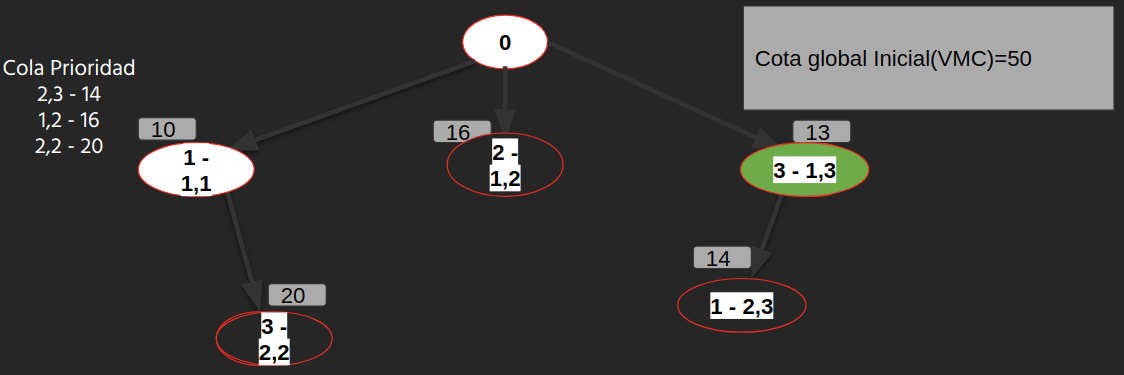
\includegraphics[width=1.0\textwidth]{./imagenes/4}
		\caption{Grafica BurbujaJava y BurbujaC} \label{fig:1}
	\end{figure}
	
	Como se puede apreciar en la gráfica, el programa BurbujaC es mas lento que el programa BurbujaJava, esto se debe a que la constante multiplicativa del termino con mayor exponente (grado 2 en este caso) de la funcion de BurbujaC es mayor que la de BurbujaJava. Para intentar representar este hecho mas fácilmente se ha realizado en la siguiente sección una ampliación del problema.\\
	
	%-----------------------------------------------------------------------
	%						Ampliacion del problema
	%----------------------------------------------------------------------	
	\section[Ampliacion del problema]{Ampliacion del problema}
	
	Para terminar vamos a realizar lo mismo que para el apartado anterior pero ahora con un tamaño a ordenar mucho mayor. Para ello se han vuelto a ejecutar ambos programas pero ahora con un tamaño de 200.000 ejecutados cada 10.000 (Un total de 20 ordenaciones).\\
	
	Después de ejecutar ambos programas se han anotado los resultados y se han introducido en la figura 2.1 .
	
	\begin{figure}[htb]
		\centering
		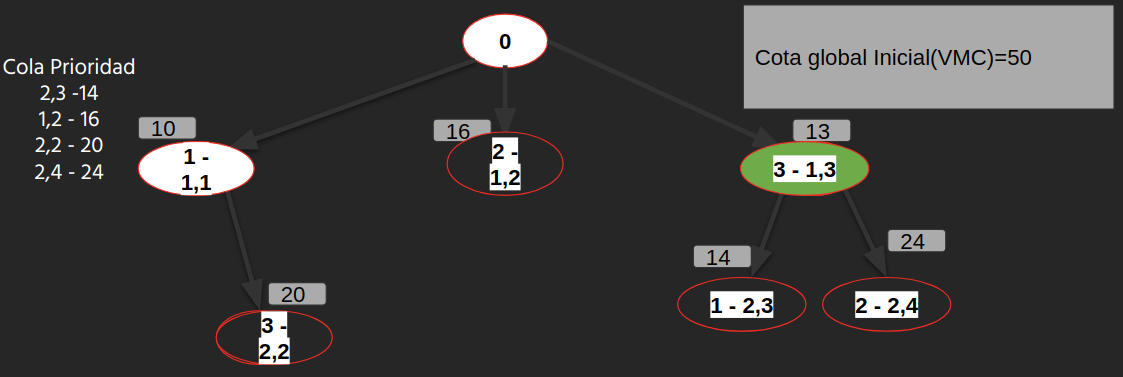
\includegraphics[width=1.0\textwidth]{./imagenes/5}
		\caption{Grafica BurbujaJava y BurbujaC con mayor tamaño N} \label{fig:1}
	\end{figure}
	
	Por ultimo , partiendo de que ambas gráficas son parábolas y su eficiencia que pertenece a O(n*n) viene sujeta a la anidación entre los blucles while y for, vamos a intentar calcular dos funciones aproximadas a las dos lineas de la gráfica. Para ello vamos a seleccionar tres puntos y a calcular la función.\\
	
	De la linea obtenida por el programa BurbujaC (color rojo) se han seleccionado los puntos:\\
	
	P1 = (0 , 0)\\
	P2 = (80.000 , 30.000)\\
	P3 = (140.000 , 90.000)\\
	
	Por lo que el sistema de ecuaciones para calcular la curva utilizando la función general de una parábola (y = a*x*x + b*x + c) sera:\\
	
	0 = a*0*0 + b*0 + c\\
	30.000 = a*80.000*80.000 + b*80.000 + c\\
	90.000 = a*140.000*140.000 + b*140.000 + c\\
	
	Por lo que al resolver el sistema de ecuaciones obtenemos que la funcion que representa la curva es :\\
	
	f(x) = (1/224000)*x*x + (1/56)x\\
	
	De la linea obtenida por el programa BurbujaJava (color azul) se han seleccionado los puntos:\\
	
	P1 = (0 , 0)\\
	P2 = (110.000 , 10.000)\\
	P3 = (180.000 , 30.000)\\
	
	Por lo que el sistema de ecuaciones para calcular la curva utilizando la función general de una parábola (y = a*x*x + b*x + c) sera:\\
	
	0 = a*0*0 + b*0 + c\\
	10.000 = a*110.000*110.000 + b*110.000 + c\\
	30.000 = a*180.000*180.000 + b*180.000 + c\\
	
	Por lo que al resolver el sistema de ecuaciones obtenemos que la función que representa la curva es :\\
	
	f(x) = 0.0000109*x*x - 0.03x\\
	
	Como conclusión obtenemos que la constante multiplicativa (aproximada) de BurbujaC (0.0000446) es mayor que la de BurbujaJava (0.0000109), por lo que los tiempos de ejecucion también son mayores.

	%-----------------------------------------------------------------------
	%							BIBLIOGRAFIA
	%-----------------------------------------------------------------------
	% Referencia a bibliografia			En \cite{Baz}
	% Referencia a figura				La figura (\ref{fig:1})
	% Espacio entre lineas				\vspace{0.06in}
	% Figura con comentario al pie
	%\begin{figure}[htb]
	%	\centering
	%	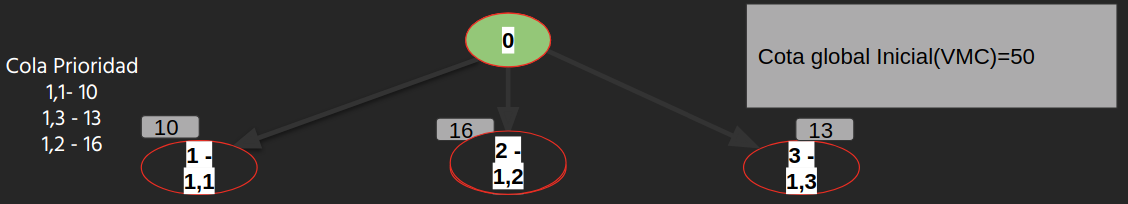
\includegraphics[width=0.4\textwidth]{./imagenes/1}
	%	\caption{Universidad de Granada.} \label{fig:1}
	%\end{figure}
	%\begin{thebibliography}{99}
	%	\bibitem{Baz} 
	%	\textsc{Bazaraa, M.S., J.J. Jarvis}
	%	\textit{Programacuib}.
	%	\newline
	%	\url{https://www.google.es}	
	%\end{thebibliography}

	


\end{document}